% Source of TAILOR_DC_SAFE_paper_zh_extended.pdf. Build in this folder with two runs of
%   xelatex -jobname=TAILOR_DC_SAFE_paper_zh_extended main.tex
% (fonts: TeX Gyre Termes/Heros, STIX Two Math, Noto Serif CJK SC) and copy TAILOR_DC_SAFE_paper_zh_extended.pdf to ../
\documentclass[a4paper,11pt]{article}
\usepackage{fontspec}
\setmainfont{TeX Gyre Termes}
\setsansfont{TeX Gyre Heros}
\newfontfamily\cjkfont{Noto Serif CJK SC}
\usepackage{amsmath}
\usepackage{unicode-math}
\setmathfont{STIXTwoMath-Regular.otf}
\usepackage[a4paper,top=2.5cm,bottom=2.4cm,left=2.6cm,right=2.6cm]{geometry}
\usepackage{graphicx,booktabs,array,threeparttable,pdfpages,fancyhdr,xurl}
\usepackage[font=small,labelsep=period,skip=4pt]{caption}
\usepackage[hidelinks,bookmarksnumbered=true,bookmarksopen=true]{hyperref}
\usepackage{titlesec}
\renewcommand{\floatpagefraction}{0.8}\renewcommand{\topfraction}{0.88}\renewcommand{\bottomfraction}{0.7}\renewcommand{\textfraction}{0.1}
\usepackage{etoolbox}\AtBeginEnvironment{thebibliography}{\small\linespread{1.05}\selectfont\setlength{\itemsep}{1pt}\setlength{\parskip}{0pt}}
\setlength{\emergencystretch}{3em}
\linespread{1.15}
\setlength{\parskip}{0.25em}
\titleformat{\section}{\large\bfseries}{E\arabic{section}}{0.8em}{}
\titleformat{\subsection}{\normalsize\bfseries}{E\arabic{section}.\arabic{subsection}}{0.6em}{}
\renewcommand{\thesection}{E\arabic{section}}
\renewcommand{\thefigure}{E\arabic{figure}}
\renewcommand{\thetable}{E\arabic{table}}
\renewcommand{\theequation}{E\arabic{equation}}
\setlength{\headheight}{15pt}\pagestyle{fancy}\fancyhf{}\renewcommand{\headrulewidth}{0.4pt}
\newcommand{\hd}[1]{\begin{tabular}[b]{@{}c@{}}#1\end{tabular}}
\newcommand{\exthead}[1]{\fancyhead[L]{\small #1}\fancyhead[R]{\small Part II\quad Post-competition extensions}\fancyfoot[C]{\small E-\thepage}}

\graphicspath{{../../figures/extension/}}
\hypersetup{pdftitle={TAILOR-DC-SAFE: compute-power co-scheduling for a green AI data centre -- extended edition}}
\begin{document}
\thispagestyle{empty}
\begin{center}
{\Large\bfseries TAILOR-DC-SAFE: Compute--Power Co-Scheduling\\[0.2em] for a Green AI Data Centre}\\[0.7em]
{\large Extended edition --- note}
\end{center}
\vspace{0.8em}

This file has two parts. Part I is the paper submitted to the Ising Intelligent Computing Future Challenge, 2026 (27 pages, in Chinese), reproduced exactly as submitted. Part II, starting on page E-1, contains post-competition extensions written in November 2026.

The paper writes the compute--power co-scheduling of 588 AI jobs as a one-of-$n$ QUBO/Ising problem, solves it by neighbourhoods on the Ising platform and a classical back end, and computes the expected cost and the CVaR$_{95}$ recourse cost by an independent multi-scenario replay. Its exact comparisons cover only controlled neighbourhoods of 30--100 jobs. E1 extends the exact MILP to all 588 jobs and obtains the proven global optimum: the submitted schedule is within 1.6\,\% of the optimum under the same peak constraint and within 2.8\,\% of the global optimum without a peak constraint. E2 explains why the Ising route stops at this gap: the QUBO energy used in the submission ranks schedules in the opposite order to the true objective, and even annealing the true objective directly, single-job moves rarely cross an energy barrier of 0.68 USD on the way to the optimum.

Every number in Part II can be reproduced with the scripts in the \texttt{extension/} folder of the code repository; result files are in \texttt{results/extension/}.

\clearpage
\pdfbookmark[0]{Part I\quad Competition paper (as submitted)}{part1}
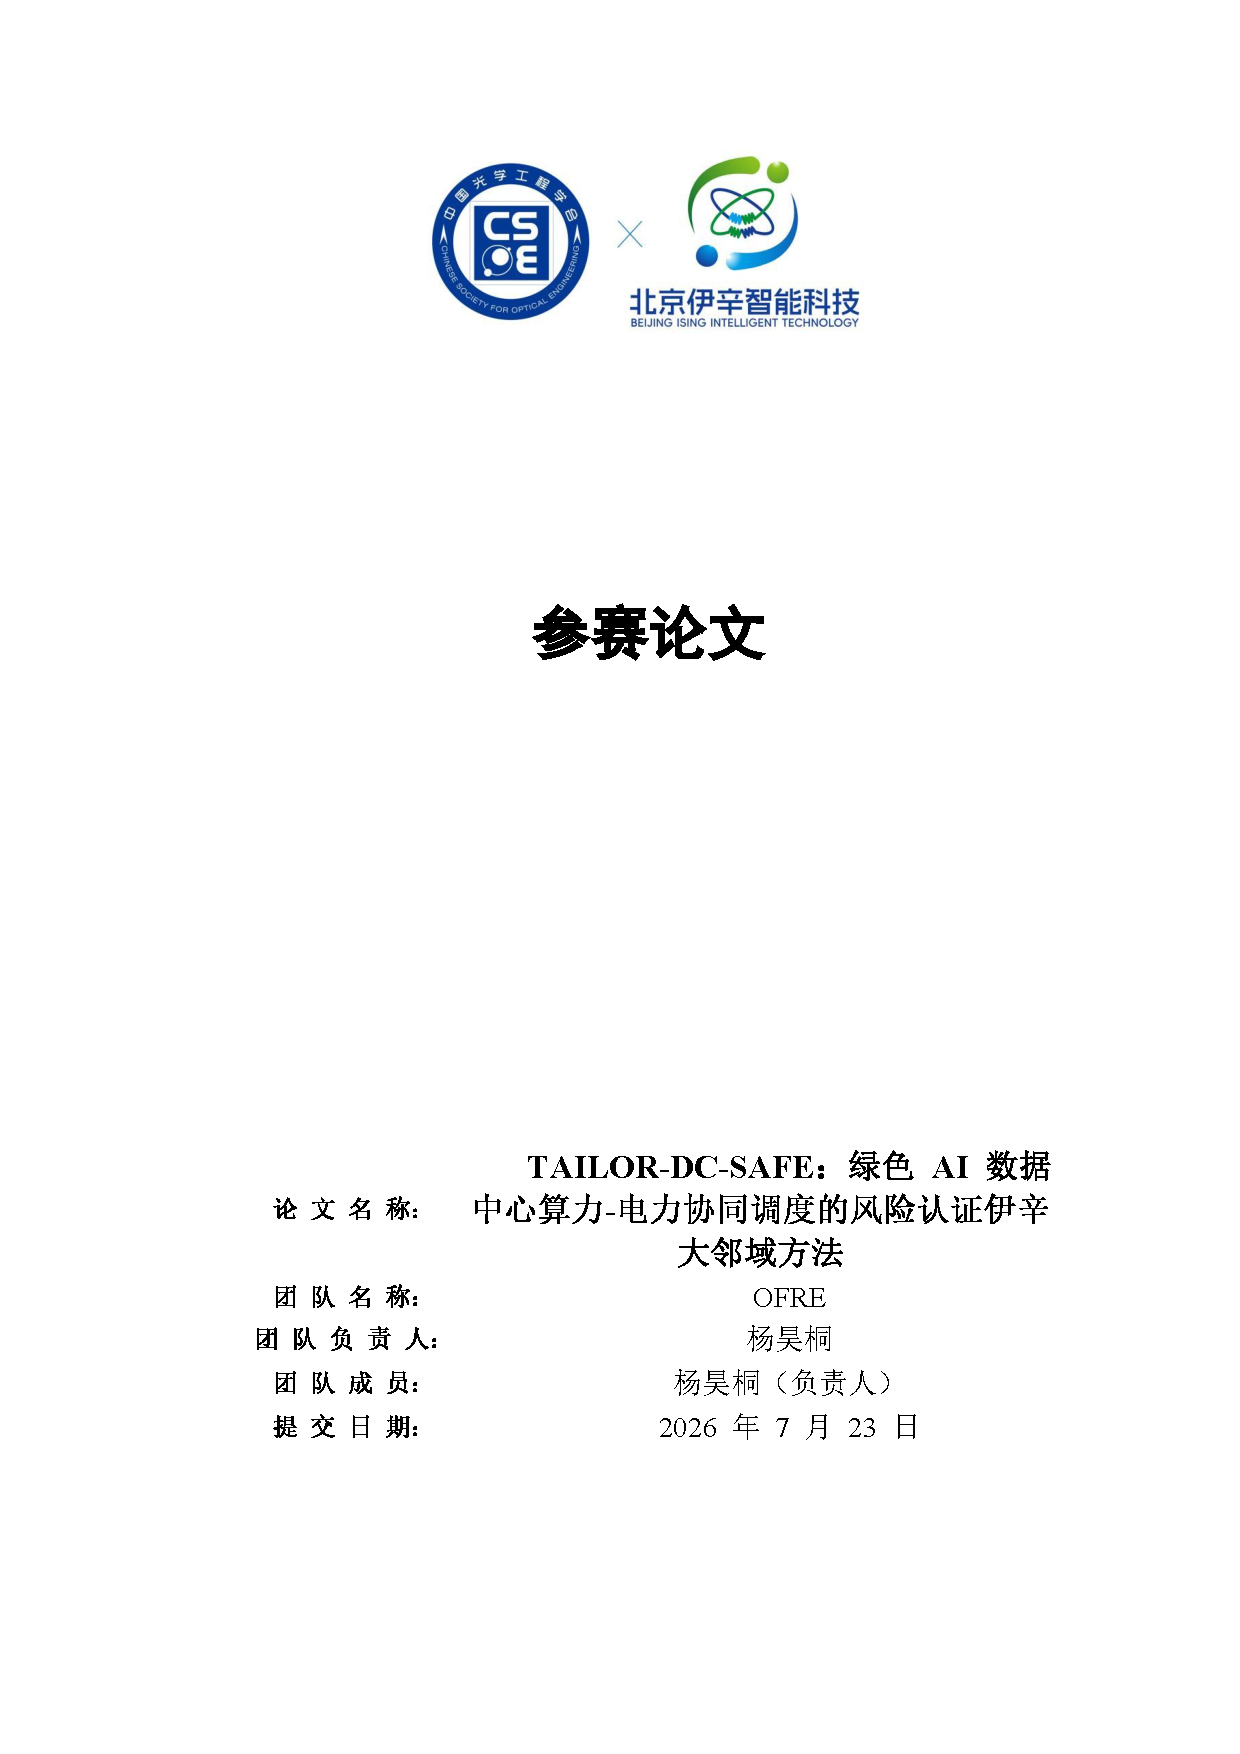
\includepdf[pages=-]{../TAILOR_DC_SAFE_paper_zh.pdf}
\pdfbookmark[0]{Part II\quad Post-competition extensions}{part2}
\setcounter{page}{1}
\exthead{TAILOR-DC-SAFE: compute--power co-scheduling}
\begin{center}{\Large\bfseries Part II\quad Post-competition extensions}\end{center}

The scheduling instance of the paper contains 588 jobs, each of which selects one of several candidate actions. The objective is the sum of the expected cost and the CVaR$_{95}$\cite{rockafellar2000} recourse cost, subject to an action-cost guard and to the IT peak load. The paper solves the QUBO form\cite{lucas2014} on the Ising platform and completes the recourse repair on the classical side. The two extensions below compute the exact optimum of the whole instance and diagnose the source of the gap between the Ising route and the optimum.

\section{An exact certificate for the whole instance}

\subsection{Model and solution}
E1 builds the exact model used by the submission for all 588 jobs: each job selects one action, the five-scenario recourse is linearised for CVaR$_{95}$, the objective is the expected cost plus CVaR$_{95}$, the action-cost guard is the same as in the submission (the minimum true action cost plus 1 USD), and dummy actions are not allowed. The model has 1\,739 variables (1\,365 of them integer) and 1\,153 constraints, and HiGHS\cite{huangfu2018} solves it to proven optimality (1.18 million branch-and-bound nodes, 22 minutes). A second solve adds the peak of the submitted schedule as a hard cap.

\subsection{Results}
\begin{table}[htbp]\centering\small\setlength{\tabcolsep}{5pt}
\caption{The submitted schedule against the exact optima (costs in USD; the objective is the sum of the expected cost and CVaR$_{95}$; the peak is the IT load peak).}\label{tab:is-e1}
\begin{tabular}{lrrrrr}\toprule
Schedule & Expected & CVaR$_{95}$ & Objective & Peak (MW) & Jobs changed\\\midrule
Submitted (QUBO/Ising + recourse repair) & 35.395 & 47.718 & 83.113 & 0.0316 & ---\\
Exact optimum, peak capped at submitted & 34.796 & 47.023 & 81.820 & 0.0316 & 224\\
Exact optimum, peak free & 34.460 & 46.414 & \textbf{80.874} & 0.0434 & 244\\\bottomrule
\end{tabular}
\end{table}

\begin{figure}[htbp]\centering
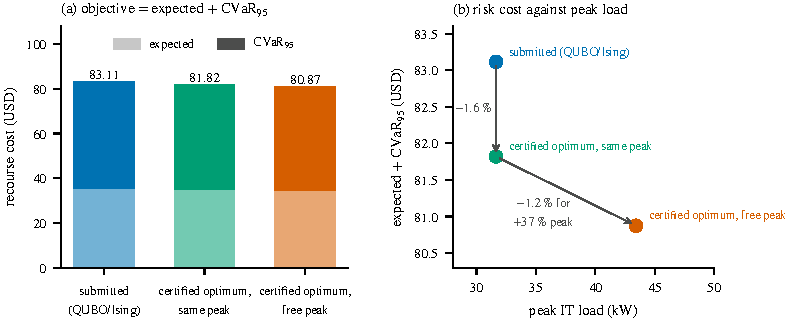
\includegraphics[width=0.82\textwidth]{figE1_exact_certificate.pdf}
\caption{(a) Composition of the objective (expected cost and CVaR$_{95}$) of the submitted schedule and of the two exact optima. (b) Trade-off between risk cost and IT peak load.}\label{fig:is-e1}
\end{figure}

The submitted schedule is within 1.6\,\% of the proven optimum at the same peak and within 2.8\,\% of the global optimum (Table~\ref{tab:is-e1}, Figure~\ref{fig:is-e1}); both gaps are now proven results rather than estimates. The last 1.2\,\% of risk cost requires a 37\,\% higher peak: the risk objective alone pushes load into cheap but concentrated periods, so the peak cap is a substantive operating constraint rather than a tie-breaker. The recourse values computed by the MILP agree with the independent evaluator to $10^{-13}$ USD, which shows that the certificate and the submitted replay measure the same objective. A third, lexicographic solve that minimises the peak among risk-optimal schedules did not finish within 25 minutes. Because the exact MILP closes the instance within half an hour on a single CPU, the honest conclusion is that instances of this size can be certified classically, and that the value of the Ising formulation lies in its neighbourhood-decomposition pipeline and its scalability to larger instances that MILP cannot close.

\section{The bottleneck of the Ising route: energy, search or landscape?}

\subsection{Design}
E1 leaves a question: why does the Ising pipeline stop 1.6--2.8\,\% above an optimum that MILP certifies in about twenty minutes? E2 compares four energy functions with the same simulated annealer. The annealer uses single-job moves that preserve the one-of-$n$ constraint and, like a constraint-preserving mixing operator, enforces the guard and the optional peak cap; every decoded schedule is scored with the exact evaluator of the submission package, and each energy is run with 8 random seeds and $12\times10^6$ candidate moves per run. The four energies are the action-cost energy of the submission (the base QUBO), a linear recourse surrogate built from period marginal costs (of the same kind as the submission's aligned-recourse family), a quadratic recourse surrogate fitted per period and corrected iteratively within a trust region, and the exact objective, which cannot be written as a QUBO.

\subsection{Results}
\begin{table}[htbp]\centering\small\setlength{\tabcolsep}{4pt}
\caption{Results of the four annealing energies (gap to the proven optimum, best / median over 8 seeds).}\label{tab:is-e2}
\begin{tabular}{lrcc}\toprule
Annealing energy & \hd{Rank agreement\\with objective} & No peak cap & \hd{Peak capped\\at submitted}\\\midrule
Action cost (base QUBO) & $-0.89$ & 23.5\,\% / 23.5\,\% & 17.7\,\% / 17.7\,\%\\
Linear recourse surrogate (marginal costs) & $-0.51$ & 4.3\,\% / 6.1\,\% & 1.6\,\% / 1.6\,\%\\
Quadratic recourse surrogate (trust region) & $\mathbf{+0.66}$ & 4.2\,\% / 4.7\,\% & 1.5\,\% / 1.5\,\%\\
Exact objective (not a QUBO) & --- & \textbf{0.39\,\% / 1.83\,\%} & \textbf{0.20\,\% / 0.44\,\%}\\
\emph{Submitted schedule} & & \emph{2.8\,\%} & \emph{1.6\,\%}\\\bottomrule
\end{tabular}
\end{table}

Rank agreement is the Spearman correlation between the energy and the exact objective along the annealing trajectories without a peak cap. Because the cheapest schedule violates the peak cap, the capped runs start from the submitted schedule.

The energy function is the first bottleneck (Table~\ref{tab:is-e2}). The base energy ranks schedules in the opposite order to the true objective, and its minimiser is exactly the cheapest schedule, 23\,\% above the optimum. The first-order recourse energy is still anti-correlated with the objective. The quadratic surrogate makes the rank agreement positive, but without a peak cap it stops 4--5\,\% from the optimum, and with the cap it only matches the submitted schedule. Search is the second bottleneck: annealing the exact objective directly with the same move set and budget gets as close as 0.2--0.4\,\% to the optimum at best, but the medians (0.4--1.8\,\%) show that single-job annealing does not reach it reliably.

\begin{figure}[htbp]\centering
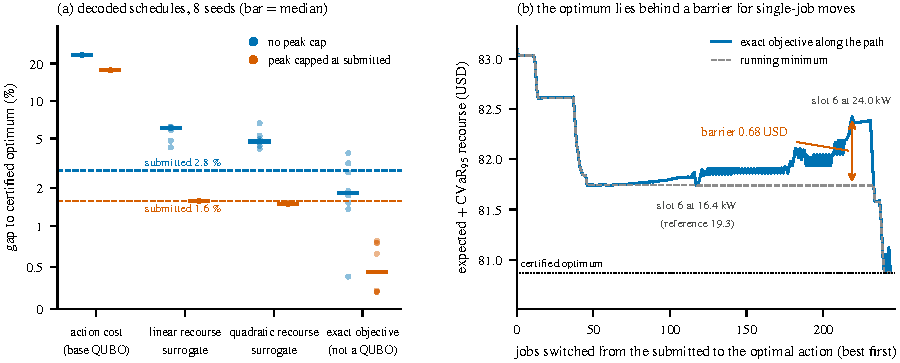
\includegraphics[width=\textwidth]{figE2_aligned_energy.pdf}
\caption{(a) Gap of the decoded schedules to the proven optimum under each annealing energy (8 seeds, horizontal lines: medians), without and with the peak cap; the dashed line marks the submitted schedule. (b) Exact objective along the greedy job-by-job path from the submitted schedule to the proven optimum.}\label{fig:is-e2}
\end{figure}

The energy landscape explains why (Figure~\ref{fig:is-e2}b). Steepest descent from the submitted schedule stops after 15 single-job moves at 83.03 USD (after 4 moves with the peak cap). On the greedy job-by-job path from the submitted schedule to the optimum (no peak cap, 244 switches), the objective first falls to 81.74 USD and must then climb by 0.68 USD: during this stretch the load of period 6 rises from 16.4 kW past its reference load of 19.3 kW to 24.0 kW. Only then does the objective fall to 80.87 USD, when period 6 reaches 29.1 kW and the number of periods above their reference load drops from 5 to 3. Once the load of a period exceeds its reference, its flexibility shortfall is capped, so piling load into a few sacrificial periods pays only after such a period is full, whereas a descent method sees only the cost increase caused by the first few jobs. (The capped path crosses the peak cap and is therefore not used.)

\subsection{Conclusions and limits}
To compete with classical methods on this problem, an Ising formulation needs two things at once: an energy that can express the kink of the recourse cost, for example through per-period, per-scenario auxiliary spins for the saturation penalty, and collective moves that shift several jobs at a time. Neither the submitted QUBO nor the smooth surrogates provide them, and at this scale MILP remains the appropriate tool. These conclusions rest on a single instance and a single annealer and do not rule out that other Ising hardware or hybrid algorithms behave differently on larger instances.

\begin{thebibliography}{9}
\bibitem{rockafellar2000} R. T. Rockafellar, S. Uryasev. Optimization of conditional value-at-risk. \emph{Journal of Risk}, 2(3): 21--41, 2000.
\bibitem{lucas2014} A. Lucas. Ising formulations of many NP problems. \emph{Frontiers in Physics}, 2: 5, 2014. doi:10.3389/fphy.2014.00005.
\bibitem{huangfu2018} Q. Huangfu, J. A. J. Hall. Parallelizing the dual revised simplex method. \emph{Mathematical Programming Computation}, 10(1): 119--142, 2018. doi:10.1007/s12532-017-0130-5.
\end{thebibliography}
\end{document}
